\chapter{Background}
\label{chap:background}

System development is a complex process, therefore it needs to be supported by various tools and algorithms. In this chapter I will introduce the background of our work \citep{tdk2015} and my previous BSc thesis \citep{bsc_thesis} towards an approach supporting correct system design.

\section{Development methods}

Traditional software development methods often use informal specifications to support system, architecture and component level designs -- which may also be informal. This can easily result in higher verification costs or faulty systems, making them suboptimal choices for safety-critical software development. In order to introduce some level of formality and allow manageable, hierarchical software testing procedures, the V model was developed.

\begin{figure}
	\centering
	\begin{tikzpicture}[
	start chain=going below,
	squarednode/.style={
		rectangle,
		draw=black,
		very thick,
		minimum height=1.5cm,
		text width=2.5cm,
		inner sep=2mm,
		align=center	
	},
	every loop/.style={
		looseness=2,
		text width=2cm	
	}
	]
	\node[squarednode] (D1) {Requirements};
	\node[squarednode] (D2) [below = of D1, xshift = 1cm] {Architecture design};
	\node[squarednode] (D3) [below = of D2, xshift = 1cm] {Component design};
	\node[squarednode] (I)  [below = of D3, xshift = 2.5cm] {Implementation};
	\node[squarednode] (V3) [above = of I , xshift = 2.5cm] {System V\&V};
	\node[squarednode] (V2) [above = of V3, xshift = 1cm] {Architecture V\&V};
	\node[squarednode] (V1) [above = of V2, xshift = 1cm] {Unit V\&V};
	\draw[thick,->] (D1) -- (D2) node [midway, left, align=right] {Refine};
	\draw[thick,->] (D2) -- (D3) node [midway, left, align=right] {Refine};
	\draw[thick,->] (D3) -- ( I) node [midway, right, align=left] {};
	\draw[thick,<-] ( I) -- (V3) node [midway, right, align=left] {};
	\draw[thick,<-] (V3) -- (V2) node [midway, right, align=left] {Use};
	\draw[thick,<-] (V2) -- (V1) node [midway, right, align=left] {Use};
	\draw[thick,->] ($(D1.east)+(0,.4)$) -- ($(V1.west)+(0,.4)$) node [midway, above] {Transform};
	\draw[thick,->] ($(D2.east)+(0,.4)$) -- ($(V2.west)+(0,.4)$) node [midway, above] {Transform};
	\draw[thick,->] ($(D3.east)+(0,.4)$) -- ($(V3.west)+(0,.4)$) node [midway, above] {Transform};
	\draw[thick,<-] ($(D1.east)-(0,.4)$) -- ($(V1.west)-(0,.4)$) node [midway, above] {Test};
	\draw[thick,<-] ($(D2.east)-(0,.4)$) -- ($(V2.west)-(0,.4)$) node [midway, above] {Test};
	\draw[thick,<-] ($(D3.east)-(0,.4)$) -- ($(V3.west)-(0,.4)$) node [midway, above] {Test};
	\end{tikzpicture}
	\caption{The traditional V model\citep{vmodel}}
	\label{fig:intro:vmodel}
\end{figure}

\cref{fig:intro:vmodel} shows the stages of development, where a symbolic ``V'' shows the progress of the workflow. The project definition stages on the left side begin with the development of a concept of operations, continue with requirements and architecture, and detailed design. The implementation stage is shown across the base of the ``V''. The right side shows the testing and implementation stages of a system, with an upward-pointing arrow for progress of the workflow\citep{vmodel}. 

The V model is the basic scheme of software development. In the left of the figure, we proceed by decomposing the specification into an architecture level design, and the architectural design into component-level designs. Every level of decomposition has it's own specification. After the implementation process, each level of the implementation is verified with respect to the corresponding specification. This verification can be done incrementally, parallel  with the implementation process.

\subsection{Model driven software development}

Model-driven software development (MDSD) emphasizes problem solving by the development and maintenance of models describing the system being designed. MDSD heavily relies on automated code and documentation generation based on the models of components or the overall model of the system. 

Modeling has the advantage of introducing abstractions, thus reducing the complexity of the development process, by dividing it into smaller phases. Code generation guarantees that the code will inherit the properties that can be directly derived from the model, while reducing the costs by eliminating unnecessary round-trip engineering. The generation of documentation also results in the always up-to-date description of components, stored together with the requirements and the model. Furthermore, model-based approaches have the advantage of easier testability, or if the model is formal enough then formal verification might be applicable. This is especially important for the development of safety-critical systems, making MDSD notably widespread in such areas.

Various methods and tools are available for the generation of test cases and monitoring components from models, as well as for formally verifying certain properties. These tools usually support the modeling formalisms used in their application domain.

MDSD will usually result in a software life cycle model for component-based systems\citep{ymodel}, which is based on the V model.

\subsection{Y model} 

\begin{figure}
	\centering
	\begin{tikzpicture}[
	start chain=going below,
	squarednode/.style={
		rectangle,
		draw=black,
		very thick,
		minimum height=1.5cm,
		text width=2.5cm,
		inner sep=2mm,
		align=center
	},
	every loop/.style={
		looseness=2,
		text width=2cm
	}
	]
	\node[squarednode] (D1) {System\\Design Model};
	\node[squarednode] (D2) [below = of D1, xshift = .2cm] {Architecture\\Design Model};
	\node[squarednode] (D3) [below = of D2, xshift = .2cm] {Component\\Design Model};
	\node[squarednode] (V1) [right = 3cm of D1] {System\\V\&V Model};
	\node[squarednode] (V2) [below = of V1, xshift = -.2cm]{Architecture\\V\&V Model};
	\node[squarednode] (V3) [below = of V2, xshift = -.2cm] {Component\\V\&V Model};
	\node[squarednode] (GC) at ($(D3)!0.5!(V3)$) [yshift=-3.5cm, text width=5.5cm] {Design + V\&V Artifacts\\(Source code, Glue code,\\Config. Tables, Test Cases,\\Monitors, Fault Trees, etc.)};
	\draw[thick,->] (D3.south) -- (GC.north -| D3) node [midway, left, align=right] {Code generation};
	\draw[thick,->] (V3.south) -- (GC.north -| V3) node [midway, right, align=left] {Test generation};
	\draw[thick,->] (D1) edge [loop left, align=right] node {Design rules} ();
	\draw[thick,->] (D2) edge [loop left, align=right] node {Design rules} ();
	\draw[thick,->] (D3) edge [loop left, align=right] node {Design rules} ();
	\draw[thick,->] (V1) edge [loop right, align=left] node {Formal methods} ();
	\draw[thick,->] (V2) edge [loop right, align=left] node {Formal methods} ();
	\draw[thick,->] (V3) edge [loop right, align=left] node {Formal methods} ();
	\draw[thick,->] (D1.south) -- (D2.north) node [midway, left, align=right] {Derive};
	\draw[thick,->] (D2.south) -- (D3.north) node [midway, left, align=right] {Derive};
	\draw[thick,<-] (V1.south) -- (V2.north) node [midway, right, align=left] {Use};
	\draw[thick,<-] (V2.south) -- (V3.north) node [midway, right, align=left] {Use};
	\draw[thick,<->] ($(D1.east)+(0,.4)$) -- ($(V1.west)+(0,.4)$) node [midway, above] {Transform};
	\draw[thick,<->] ($(D2.east)+(0,.4)$) -- ($(V2.west)+(0,.4)$) node [midway, above] {Transform};
	\draw[thick,<->] ($(D3.east)+(0,.4)$) -- ($(V3.west)+(0,.4)$) node [midway, above] {Transform};
	\draw[thick,<->] ($(D1.east)-(0,.4)$) -- ($(V1.west)-(0,.4)$) node [midway, above] {Test};
	\draw[thick,<->] ($(D2.east)-(0,.4)$) -- ($(V2.west)-(0,.4)$) node [midway, above] {Test};
	\draw[thick,<->] ($(D3.east)-(0,.4)$) -- ($(V3.west)-(0,.4)$) node [midway, above] {Test};
	\end{tikzpicture}
	\caption{An overview of the Y model}
	\label{fig:intro:ymodel}
\end{figure}

The Y model\citep{ymodel} is an extension of the V model\citep{randomwikipedialink3}, by automating code and test case generation. Much like the V model, the development process is partitioned vertically. Each level has its own modeling languages and models that are transformed to a verification model, on which verification methods such as testing can be applied. The results of the verification process can be traced back to the original models making iterative improvement possible. The top level is for high level system models, while the second level contains architectural models, and the third one is for component-based models. The component model provides input for the source code and configuration generation for the individual components. Test cases are paired with the source code and can be generated from the component verification models.


\subsection{Modeling languages on different levels of abstraction}

Model Driven Software Development methods require modeling languages to describe the behavior of systems and components. Engineering practices resulted a wide range of such languages over the years to support efficient product development. This allows the use of domain-specific languages, which leads to a shorter modeling process. The result is the need for complex model transformations before the verification can begin,
but since the domain-specific languages are tailored exactly to the problem, their usage is more efficient -- but requires expertise in the domain.  

Standardized modeling languages were developed like the UML (Unified Modeling Language\citep{uml}) and SysML (Systems Modeling Language\citep{sysml1}\citep{sysml2}).

\subsubsection{Class diagram}

In software engineering, a class diagram in the Unified Modeling Language (UML) is a type of static structure diagram that describes the structure of a system by depicting the system's classes, their attributes, operations (or methods), and the relationships among objects. It is also often applied at the system level design, as multiple components and their connection can be visualized with Class diagrams.

\subsubsection{Message Sequence Chart}

The formalism of Message Sequence Charts (MSC) describes the communication between components -- the order in which messages can occur\citep{msc}\citep{msc2}\citep{Klose2003}. The message interchange is usually represented by a graphical model. These charts can be used for high-level specification, design, trace-based testing or documentation. A collection of possible sequence charts can also describe a complete communication protocol between components. UML sequence diagrams were inspired by MSCs, but their semantics differs regarding some of the basic elements of the language such as lifelines and arrows\citep{mscuml}.

\subsubsection{Sequence diagram}

A Sequence Diagram is an interaction diagram that shows how processes operate with one another and in what order. It is a construct of a Message Sequence Chart. A Sequence Diagram shows object interactions arranged in time sequence. It depicts the objects and classes involved in the scenario and the sequence of messages exchanged between the objects needed to carry out the functionality of the scenario. Sequence diagrams are typically associated with use case realizations in the logical view of the system under development. Sequence diagrams are sometimes called event diagrams or event scenarios. Sequence diagrams can be used for system-level modeling, as it can represent the communication between the components. 


\subsubsection{Statechart}

Statecharts, also known as state machines are an extension of finite automata. There are various available syntaxes for statecharts (e.g. the one defined by UML\citep{stcuml}). The higher level concepts that were introduced include variables, actions, and hierarchically nested states. Event-driven execution is also possible by using signals as the triggers of transitions. Available variable types heavily depend on the concrete semantics of the chosen statechart language. Actions can usually be variable assignments, signal raises or the setting of timers. Hierarchy lets users organize system descriptions using a top-down approach. Support for hierarchy is introduced via nested states and parallel regions. States can also have entry and exit actions, which allows the description of common functionality in parent states\citep{stcmove}.%\\

Statecharts are usually developed in tools that support the graphical design of the model (e.g.: Yakindu\citep{yakinduu}, an Eclipse-based editor).
Statecharts are commonly used as a form of component description, as it can represent the behavior of components depending on its state.

\subsubsection{Activity Diagram}

Activity diagrams are graphical representations of workflows of stepwise activities and actions with support for choice, iteration and concurrency. In the Unified Modeling Language, activity diagrams are intended to model both computational and organizational processes (i.e. workflows). Activity diagrams show the overall flow of control, and therefore can be used at the system level description.

\section{Verification techniques} 

As modern society is becoming more and more dependent on safety-critical systems, the need for faultlessly working hardware and software increases. The development of safety-critical systems require extensive testing efforts. Validation and verification methodologies have been present in the development processes of such systems for a long time\citep{ieee1012}, but faster and more reliable approaches are needed. Validation assures that the requirements specified for the software meet the needs of the user -- as such, validation usually can be aided, but can’t entirely be done by software. The goal of verification is to analyze whether the specified requirements are met by the system. Methods for verification can be divided into two groups: design time verification and runtime verification. These approaches aren't exclusive, and their mutual use can support a more robust verification process.

\subsection{Design time verification}

Design time verification is a method used for finding errors of the system before deployment. Traditional software development methodologies usually rely on design time approaches. Verification methods can be applied on multiple levels, from small parts to the whole system. These processes check the compliance of the system against the specification of the appropriate level.%\\ \todo{This line break is strange}

Formal verification can also be used to give proof that the verified parts match the behavior described by the (also formal) specification. On the other hand, applying formal methods usually have higher costs, and the verification of complex systems can be impossible due to the phenomenon of state space explosion. As a result, a possible application of formal methods is to verify the correct behavior of system components, and not the entire system.

\subsection{Runtime verification}

Runtime verification is a method for the inspection of running systems. The motivation of the approach
is to reduce to complexity of the design time verification. 
As systems are getting larger, the application of formal methods are more and more limited as the resources needed for verification cannot be realized. This means that formal verification methods must verify an abstract model, not the deployed system itself. In addition, specifications are rarely complete, and design time methods can rarely handle hardware errors. %\todo{This line break is strange}

Runtime verification uses monitors to observe certain (usually critical) components, checking whether their operation violates properties described in the specification. The usage of monitoring components can result in significantly smaller monitors than the component itself as multiple levels of abstraction can be used, as long as the error states remain distinguishable. This has the advantage of detecting the erroneous operation of the system and allows systematic safety engineering to handle faults, or trigger an emergency shutdown if necessary.

The main advantages of runtime verification are the following:

\begin{itemize}
	\item Smaller computational complexity.
	\item Verification of the running implementation.
	\item Detection of previously not defined errors.
\end{itemize}

\section{Complex event processing}

\begin{figure}[h]
	\centering
	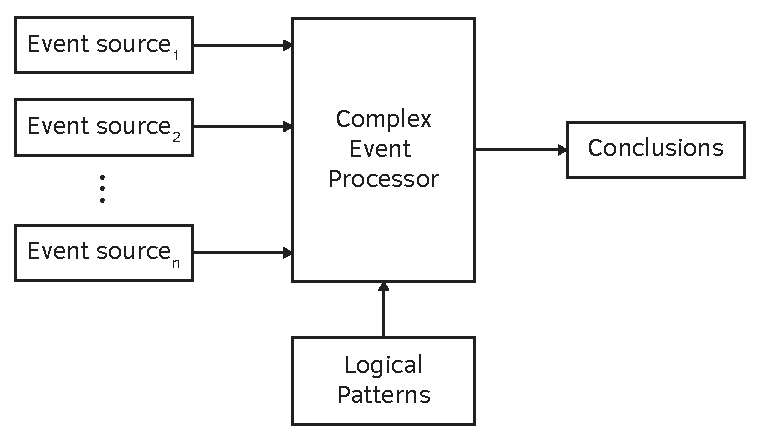
\includegraphics[width=0.6\linewidth]{figures/chapter_2/CEP}
	\caption{Complex event processing overview \redraw }
	\label{fig:intro:cep}
\end{figure}

Complex event processing (or CEP for short) is a method of tracking and analyzing streams of information and deriving conclusions. In a complex event processing environment, there can be multiple event sources, and with logical patterns given by a formalism, patterns (pattern matches) can be found in the incoming stream, e.g.~events followed by another events in some predefined sequence.

\subsection{Complex Event Processing Frameworks}
There are many Complex Event Processing Frameworks in the industry.

One of these tools is Drools\citep{drools} which is the leading Java based open-source rule engine. It is a hybrid chaining engine meaning that it can react to changes in data and also provides advanced query capabilities. Drools provides built-in temporal reasoning for complex event processing and is fully integrated with the jBPM project for BPMN2 based workflows.

Another well-known tool in the industry is Esper\citep{esper} which is an Event Stream Processing (ESP) and event correlation engine.
Targeted to real-time Event Driven Architectures (EDA), Esper is capable of triggering custom actions written as Plain Old Java Objects (POJO) when event conditions occur among event streams. It is designed for high-volume event correlation where millions of events coming in seconds. This amount of input would make it impossible to store all event in a classical database architecture and query them later.

\section{Runtime verification with CEP}
In this section the application of CEP for runtime verification is overviewed.
In general, system level runtime verification can be provided with the help of complex event processing. A complex event processing framework can monitor either the messaging between components and also the current state of the system and detect errors based on the specification of valid message sequences and valid states. 
The approach uses pattern matching to detect faulty operation of the system. Should illegal sequences occur, error handling operations (e.g.~restart or shutdown of a component or the whole system) can be applied to avoid the violation of safety criteria.

\subsection{Finite automaton }

\todo{How the fuck did this get here?}
The modeling of systems with finite state space is often done by using finite automata -- also known as finite state machines. A finite automaton accepts a (finite) list of symbols and produces a computation of the automaton for each input list.
Although finite automata can be easily visualized, this formalism describes a simple, flat transition system and lacks the support for higher level concepts. The development of finite automata models are supported by many tools (e.g.: Finite State Machine Designer \citep{fsmd}).

\subsection{Data structures supporting parametric decision}
Most of the Complex Event Processing tools support the handling of parameters, such as parametric events.
To support such functionalities, some data structure is required which can decide which parameters are in them and which of them are not.

\subsubsection{BDD and MDD}

Many problems can be stated naturally using variables that have multiple values (i.e., take their values from a discrete domain). Functions defined on these variables can also take on values from a discrete set. Examples of such problems range from combinatorial optimization such as routing and resource scheduling, to logic simulation and formal verification, and to logic synthesis such as state minimization and state assignment. In many cases these problems are NP-complete or coNP-complete. Compact representation and efficient manipulation of such multi-valued functions are key to the design of efficient algorithms that advance the frontier of the problems that can be solved exactly. Binary decision diagrams (BDDs) are such a compact representation for problems involving binary variables. In this paper, we define the multi-valued decision diagram (MDD), which is a canonical representation of a multi-valued function as a directed acyclic graph. We analyze its properties and provide algorithms for constructing and manipulating MDDs. With our MDD package, an MDD is mapped into a BDD using either a logarithmic encoding or a 1-hot encoding, each suitable for a different class of applications. We have applied both kinds of MDD to many different applications, and this paper serves as a summary of the work done so far. Furthermore, general problem solving techniques, such as binate table covering and other graph algorithms, have been formulated using MDDs.\citep{Kam98mdd}

\subsubsection{BDD}

\todo{Steal an abstract and add a reference? Or the previous is enough?}

\subsubsection{Trie}


\todo{Steal an abstract and add a reference}

\section{Model based tools}
In this section I introduce the basic model-based tools and technologies I used in my work. The motivation of using models, and model-based technologies are:
\begin{itemize}
	\item The models can be formal, or can be transformed into a formal model, and formal models can be formally verified.
	\item A model is a high-level representation of a software component, allowing us to use a high level of abstraction in the implementation and the documentation as well.
\end{itemize}

\subsection{Eclipse Modeling Framework}
The EMF project is a modeling framework and code generation facility for building tools and other applications based on a structured data model. From a model specification described in XMI, EMF provides tools and runtime support to produce a set of Java classes for the model, along with a set of adapter classes that enable viewing and command-based editing of the model, and a basic editor. EMF (core) is a common standard for data models, many technologies and frameworks are based on. This includes server solutions, persistence frameworks, UI frameworks and support for transformations.

EMF consists of three fundamental pieces:
\begin{itemize}
	\item \textbf{EMF} -- The core EMF framework includes a metamodel (Ecore) for describing models and runtime support for the models including change notification, persistence support with default XMI serialization, and a very efficient reflective API for manipulating EMF objects generically.
	\item \textbf{EMF.Edit} -- The EMF.Edit framework includes generic reusable classes for building editors for EMF models.
	\item \textbf{EMF.Codegen} -- The EMF code generation facility is capable of generating everything needed to build a complete editor for an EMF model. It includes a GUI from which generation options can be specified, and generators can be invoked. The generation facility leverages the JDT (Java Development Tooling) component of Eclipse\citep{EMF}.
\end{itemize} 

EMF metamodels (or EMF class diagrams) are similar to UML class diagrams, a node represents a classifier, and the edges are associations or containments, depending on their endings.
Also note, that
EMF class diagrams are manipulating an EMF model and they use the genmodel package to generate Java code but
UML class diagram represents directly a Java model in UML.

\subsection{VIATRA}
The VIATRA framework supports the development of model transformations with specific focus on event-driven, reactive transformations and offers a language to define transformations and a reactive transformation engine to execute certain transformations upon changes in the underlying model. Furthermore, the underlying incremental query engine, originating from the EMF-IncQuery project is reusable in different scenarios not related to model transformations.\citep{VIATRA}

VIATRA-Query is a query language in the VIATRA framework for defining declarative graph queries over EMF models, and executing them efficiently without manual coding in an imperative programming language such as Java\citep{IncQuery}.

Graph  patterns are  an  expressive  formalism used for various purposes in Model Driven Development,  such  as  the definition of  declarative  model transformation  rules,  defining  the  behavioral  semantics of dynamic domain-specific languages, or capturing general purpose model queries including model validation constraints. A graph pattern (GP) represents  conditions  (or  constraints)  that  have  to be fulfilled by a part of the instance model. A basic graph pattern consists of structural constraints prescribing the existence of nodes and edges of a given type. Languages usually include a way to express attribute constraints. A negative application condition (NAC) defines cases when the original pattern is not valid (even if all other constraints are met), in form of a negative sub-pattern. With NACs nested in arbitrary depth, the expressive power of graph patterns is equivalent to first-order logic. A match of a graph pattern is a group of model elements that have the same configuration as the pattern, satisfying all the constraints (except for NACs, which must be made unsatisfiable)\citep{bergmann2010incremental}.


\subsection{VIATRA-CEP}
CEP plays an important role in model-driven engineering (MDE) as a supporting technique in various scenarios. The VIATRA project delivers a state-of-the-art event processing framework for the MDE scene, called VIATRA-CEP\citep{CEP}. 

The VIATRA-CEP is using the EMF models, and the VIATRA-Query graph search engine to deliver a high throughput, model-based complex event processing framework.

I will introduce more details about VIATRA-CEP in~\cref{chap:viatra_cep}.


\todo{New related work?}

\section{Related work}
\todo{This is actually not related work, maybe remove this?}
Runtime verification has a long-standing history and it is applied in various domains.
Starting from analyzing the runs of the processors by special constructs called watchdog processor up to the system level verification of whole hardware--software ecosystems with the help of CEP.
Various languages were designed to specify the requirements.
% \paragraph{Linear Temporal Logic}
Linear temporal logic (LTL) is a popular formalism for the specification and
verification of concurrent and reactive systems\citep{pnueli1977temporal}.
Most approaches that use LTL adopt a discrete model of time, where a run of a system produces a sequence
of observations. Such a model is inadequate for real-time systems, where a run
of a system is modelled either as a sequence of events that are time-stamped
with reals or as a trajectory with domain the set $\mathbb{R}_+$ of non-negative reals\citep{nivckovic2010mtl}.
% \paragraph{Metric Temporal Logic}

Current approaches to monitoring real-time properties suffer either from unbounded space requirements or lack of expressiveness. In paper~\citep{ho2014online} the authors adapted a separation technique to enable  the rewriting of arbitrary MTL formulas into LTL formulas over a set of atoms comprising bounded MTL formulas. As a result, they obtain the first trace-length independent online monitoring procedure for full MTL in a dense-time setting.

Web  service  applications  are  distributed  processes  that  are  composed  of  dynamically  bounded  services.  In paper~\citep{simmonds2013monitoring}  the authors  give  a  definitive description  of  a  framework  for  performing  runtime  monitoring  of  web  service applications against behavioral correctness properties described as finite	state  automata.  These  properties  specify  forbidden  and  desired  interactions	between service partners. Finite execution traces of web service applications described in BPEL are checked for conformance at runtime. When violations	are discovered, our framework automatically proposes adaptation strategies,	in the form of plans, which users can select for execution. Our framework also allows verification of stated pre- and post-conditions of service partners and provides guarantees of correctness of the generated recovery plans.

%hw
In ultra-critical systems, even if the software is fault-free, because of the inherent unreliability of commodity hardware and the adversity of operational environments, processing units (and their hosted software) are replicated, and fault-tolerant algorithms are used to compare the outputs. The authors of~\citep{pike2012runtime} investigate both software monitoring in distributed fault-tolerant systems, as well as implementing fault-tolerance mechanisms using RV techniques. They describe the Copilot language and compiler, specifically designed for generating monitors for distributed, hard real-time systems, and they describe a case study in a Byzantine fault-tolerant airspeed sensor system.

%hw2 es nyelv
Paper~\citep{reinbacher2011past} presents  a  method  for  runtime  verification  of microcontroller binary code based on past time linear temporal logic(ptLTL).  The authors  show  how  to  implement  a  framework  that,  owing  to  a	dedicated hardware unit, does not require code instrumentation, thus,		allowing the program under scrutiny to remain unchanged. Furthermore, they demonstrate techniques for synthesizing the hardware and software units required to monitor the validity of	ptLTL specifications.

PSL is a property specification language recently standardized as IEEE 1850TM-2005 PSL. It includes as its temporal layer a linear temporal logic that enhances LTL with regular expressions and other useful features. PSL and its precursor, Sugar, have been used by the IBM Haifa Research Laboratory for formal verification of hardware since 1993, and for informal (dynamic, simulation runtime) verification of hardware since 1997. More recently both Sugar and PSL have been used for formal, dynamic, and runtime verification of software. In paper`\citep{eisner2007psl} the authors introduced PSL and briefly touch on theoretical and practical issues in the use of PSL for dynamic and runtime verification.

A goal of runtime software-fault monitoring is to observe software behavior to determine whether it complies with its intended behavior. Monitoring allows one to analyze and recover from detected faults, providing additional defense against catastrophic failure. Although runtime monitoring has been in use for over 40 years, there is renewed interest in its application to fault detection and recovery, largely because of the increasing complexity and ubiquitous nature of software systems.\citep{delgado2004taxonomy}
